\documentclass{article}
\usepackage{arxiv}
\usepackage[utf8x]{inputenc}
\usepackage[english, russian]{babel}
\usepackage[T2A, T1]{fontenc}
\usepackage{url}
\usepackage{booktabs}
\usepackage{amsfonts}
\usepackage{nicefrac}
\usepackage{microtype}
\usepackage{lipsum}
\usepackage{graphicx}
\usepackage{natbib}
\usepackage{doi}
\usepackage{amsmath,amsfonts,amssymb,amsthm,mathtools}
\usepackage{caption}
\usepackage{float}
\usepackage{subcaption}

%\usepackage{subfigure}
\DeclareMathOperator*{\argmax}{\arg\!\max}
\DeclareMathOperator*{\argmin}{\arg\!\min}



\title{Ускорение семплирования из диффузионных моделей с использованием состязательных сетей}

\author{Охотников Н. В.\\
	\texttt{okhotnikov.nv@phystech.edu} \\
	\And
    Исаченко Р.В. \\
	\texttt{isa-ro@yandex.ru} \\
}
\date{}

\renewcommand{\shorttitle}{\textit{arXiv} Template}

%%% Add PDF metadata to help others organize their library
%%% Once the PDF is generated, you can check the metadata with
%%% $ pdfinfo template.pdf
\hypersetup{
pdftitle={A template for the arxiv style},
pdfsubject={q-bio.NC, q-bio.QM},
pdfauthor={Охотников Н.В., Исаченко Р.В.},
}
\begin{document}
\maketitle
\begin{abstract}
	В последние годы широкое распространение получили диффузионные генеративные модели, показывающие высокое качество получаемых семплов и хорошее покрытие исходного распределения. Главный их недостаток -- скорость семплирования: для получения одного объекта требуется от сотен до тысяч итераций. Активно исследуются способы ускорения этого процесса. В работе анализируется один из таких способов -- использование состязательных моделей для сокращения числа шагов, необходимых для получения семпла. Предлагается развить идею представленной ранее модели Denoising Diffusion GAN. Рассматриваются альтернативные варианты задания сложного распределения в обратном диффузионном процессе, анализируется скорость работы и качество получаемых семплов.
\end{abstract}

\section{Введение}
 После того, как была представлена Denoising Diffusion Probabilistic Models (DDPM) \cite{https://doi.org/10.48550/arxiv.2006.11239} модели на ее основе становились все популярней, показывая лучшее или сравнимое со state-of-the-art состязательными сетями \cite{https://doi.org/10.48550/arxiv.1812.04948} качество генерации\cite{https://doi.org/10.48550/arxiv.2105.05233}, при значительно более простом процессе обучения и более широком покрытии исходного распределения. Несмотря на это, использование диффузионных моделей на практике часто слишком дорого, ввиду необходимости запуска сети до 2000 раз для генерации каждого семпла. Предлагались различные способы ускорения этого процесса \cite{https://doi.org/10.48550/arxiv.2102.09672}, многие из которых обобщены в FastDDPM \cite{https://doi.org/10.48550/arxiv.2106.00132}, но большинство из них все еще требуют многих десятков итераций и не позволяют приблизиться к состязательным сетям по скорости генерации. В данной работе исследуется проблема дальнейшего ускорения семплирования.
 
 Основное предположение для большинства диффузионных моделей -- нормальность условного распределения следующего шага по предыдущему в обратном процессе. Это достигается лишь в приближении бесконечно малых во времени шагов, а значит на практике требует достаточного большого количества итераций. Для того, чтобы обойти это предположения необходимо уметь приближать сложное мультимодальное распределение, ведь каждому шумовому семплу соответствует целое множество семплов из исходного распределения. Одним из способов это реализовать является использование неявных генеративных моделей, например GAN, на каждом шаге обратного диффузионного процесса. В одной из работ \cite{https://doi.org/10.48550/arxiv.2112.07804} уже была представлена модель Denoising Diffusion GAN, реализовавшая эту идею. Подобный подход позволил снизить необходимое количество шагов до нескольких единиц и добиться ускорения семплирования на 2 порядка в сравнении с оригинальной DDPM. 
 
 В работе предлагается воспроизвести и развить результат описанный в оригинальной статье про DDGAN \cite{https://doi.org/10.48550/arxiv.2112.07804}. Основной рассматриваемой идеей является использование неявных генеративных моделей для восстановления исходного распределения. В качестве модели рассматривается GAN с различными схемами тренировки. Изучается влияние постановки оптимизационной задачи для состязательной сети на качество получаемых семплов в зависимости от числа шагов обратного диффузионного процесса.
 
 
 \section{Аппроксимация обратного диффузионного процесса мультимодальными распределениями}
 \subsection{Дифузионные модели}
 В стандартных дифузионных моделях \cite{https://doi.org/10.48550/arxiv.1503.03585, https://doi.org/10.48550/arxiv.2006.11239} рассматриваются прямой и обратный диффузионные процессы. Модель получает на вход сэмпл из исходного распределения $\mathbf{x_0}\sim q(\mathbf{x})$ и в течение $T$ шагов создает зашумленные его версии $\mathbf{x_1}\dots \mathbf{x_T}$ по следующему правилу:
 \begin{equation}
 	q(\mathbf{x_t}|\mathbf{x_{t-1}}) = \mathcal{N}(\mathbf{x_t}; \sqrt{1-\beta_t}\mathbf{x_{t-1}}, \beta_t \mathbf{I}),
 \end{equation}
где $\{\beta_t \in (0, 1)\}_{t=1}^T$. Откуда принимая $\alpha_t = 1 - \beta_t,~~\overline{\alpha_t} = \prod_{i=1}^t \alpha_i$:
 \begin{equation}
	q(\mathbf{x_t}|\mathbf{x_0}) = \mathcal{N}(\mathbf{x_t}; \sqrt{\overline{\alpha_t}}\mathbf{x_0}, (1-\overline{\alpha_t})\mathbf{I}).
\end{equation}

При достаточно больших $T$ со сколько угодно большой точностью $\mathbf{x}_T\sim \mathcal{N}(0,\mathbf{I})$. Таким образом, прямой диффузионный процесс за большое число шагов, добавляя на каждом некоторый нормальный шум, сводит сэмпл из исходного распределения к сэмплу из стандартного нормального. 

Пусть $\mathbf{X} = (\mathbf{x_0^1}\dots \mathbf{x_0^n})\sim p_0(\mathbf{x})$ -- обучающая выборка, т.е. некоторые семплы из распределения, объекты которого модель должна научиться генерировать. $p(\mathbf{x_1}\dots \mathbf{x_T}) = p_\theta(\mathbf{x_T})p_\theta(\mathbf{x_{T-1}}|\mathbf{x_T})\dots p_\theta(\mathbf{x_0}|\mathbf{x_1})$ -- совместное распределение генерируемых на каждом шаге обратного процесса объектов, $\theta$ -- обучаемые параметры модели. Тогда для построения обратного процесса воспользуемся методом максимального правдоподобия:
 \begin{equation}
	\theta^* =\argmax\limits_{\theta} p(\mathbf{X}|\theta) = \argmax\limits_{\theta} \sum\limits_{i=1}^n \log{p(\mathbf{x_0^i}|\theta)},
\end{equation}

 \begin{equation}	
	 \sum\limits_{i=1}^n \log{p(\mathbf{x_0^i}|\theta)}\geqslant \sum\limits_{i=1}^n \mathcal{L}(\theta, q;\mathbf{x^i_0}) = \sum\limits_{i=1}^n\int q(\mathbf{x_1}\dots \mathbf{x_T})\log{ \frac{p(\mathbf{x_0^i},\mathbf{x_1}\dots \mathbf{x_T})}{q(\mathbf{x_1}\dots \mathbf{x_t}|\mathbf{x_0^i})}}d\mathbf{x_1}\dots \mathbf{x_T}.
\end{equation}
 Неравенство обосновано в \cite{https://doi.org/10.48550/arxiv.1312.6114}. Подставляя в правую часть известные из прямого процесса распределения и пользуясь формулой Байеса получаем, что для максимизации правой части требуется (см. \cite{https://doi.org/10.48550/arxiv.2006.11239}) минимизировать следующее выражение:
 \begin{equation}
 	 	\label{KL_loss}
	\sum\limits_{t=1}^n \mathbb{E}_{\mathbf{x_1}\dots \mathbf{x_T}} KL\left(q(\mathbf{x_{t-1}}|\mathbf{x_t}, \mathbf{x_0})~||~p_\theta(\mathbf{x_{t-1}}|\mathbf{x_t})  \right).
\end{equation}
Для стандартной диффузионной модели после этого шага $p_\theta(\mathbf{x_{t-1}}|\mathbf{x_t})$ принимается нормальным, что очевидно из теоремы Байеса в приближении малости шага, тогда KL-дивергенция существенно упрощается и после правильной параметризации $p_\theta(\mathbf{x_{t-1}}|\mathbf{x_T})$ получаем итоговое выражение, которое оптимизируется в модели:
 \begin{equation}
	L(\theta) =  \sum\limits_{i=1}^n \sum\limits_{t=2}^n \frac{\beta^2}{2\overline{\beta_t} (1-\beta)(1-\overline{\alpha_t})} ||\varepsilon - \widehat{\varepsilon_\theta}(\mathbf{x_t^i}, t)||^2\longrightarrow\min\limits_\theta,
\end{equation}
где 
 \begin{equation*}
	\overline{\beta_t} = \frac{1-\overline{\alpha_{t-1}}}{1 - \overline{\alpha_t}}, ~~~~~~~~ \widehat{\varepsilon_\theta}(\mathbf{x_t^i}, t) = \frac{\mathbf{x_t^i} - \sqrt{\overline\alpha_t} \mathbf{x_0^i}}{\sqrt{1-\overline\alpha_t}}.
\end{equation*}

 \subsection{Мультимодальные распределения}
Итак, мы показали, что требование к большому количеству итераций в диффузионных моделях вытекает из предположения нормальности $p_\theta(\mathbf{x_{t-1}}|\mathbf{x_t})$, необходимого для подсчета $KL$-дивергенции. Однако, это распределение также может быть проинтерпретировано 
как $p_\theta(\mathbf{x_{t-1}}|\mathbf{x_t}) = q(\mathbf{x_{t-1}}|\mathbf{x_t},\mathbf{x_0} = f_\theta(\mathbf{x_t}, t))$, т.е. как предсказание $\mathbf{x_0}$ некоторой моделью, зависящей от времени и последующее зашумление его до семпла из $q(\mathbf{x_{t-1}}|\mathbf{x_t},\mathbf{x_0})$ с помощью известных из прямого прохода переходов. Таким образом, если уметь аппроксимировать некоторое сложное мультимодальное распределение (одному зашумленному семплу соответствует целое множество из исходного распределения), то можно достичь поставленной цели -- значительно сократить количество итераций обратного прохода. 
\subsection{DDGAN}
Одним из возможных подходов для этого является использование состязательных сетей. В таком случае обратный процесс устроен следующим образом: для каждого времени $t$ из объектов $\{\mathbf{x_t^i}\}$с помощью генератора получаем сэмплы $\{\mathbf{x_0^i}\}$ из исходного распределения, последовательно добавляя шум получаем $\mathbf{x_{t-1}^i}$, и применяем дискриминатор к парам из $\mathbf{x_{t-1}^i}$ и истинных зашумленных объектов из прямого прохода $\{\mathbf{\widehat{x_t^i}}\}$, который обучается определять, являются ли $\mathbf{x_{t-1}^i}$ правдоподобными <<расшумленными>> версиями $\{\mathbf{\widehat{x_t^i}}\}$. 

Подставляя в \ref{KL_loss} вместо $KL$-дивергенции метрику Васерштейна, дивергенцию Йенсена-Шеннона, f-дивергенцию и другие функции, использующиеся в различных подходах к обучению GAN моделей \cite{https://doi.org/10.48550/arxiv.1406.2661, 
		https://doi.org/10.48550/arxiv.1701.07875,
		https://doi.org/10.48550/arxiv.1606.00709,
		https://doi.org/10.48550/arxiv.2010.08029} 
как $D_{adv}$
получаем следующую задачу минимизации:
 \begin{equation}
	\min\limits_\theta\sum\limits_{t\geqslant 1}^n \mathbb{E}_{q(\mathbf{x_t})}[ D_{adv}\left(q(\mathbf{x_{t-1}}|\mathbf{x_t}, \mathbf{x_0})~||~p_\theta(\mathbf{x_{t-1}}|\mathbf{x_t})  \right)]
\end{equation}
Зададим дискриминатор от параметров $\varphi$ как $D_\varphi(\mathbf{x_{t-1}}, \mathbf{x_t}, t)$ и рассмотрим для начала non-saturating GAN \cite{https://doi.org/10.48550/arxiv.1406.2661}, в таком случае дискриминатор будем тренировать на минимизацию следующего выражения:
 \begin{equation}
	\min\limits_\varphi\sum\limits_{t\geqslant 1}^n \mathbb{E}_{q(\mathbf{x_t})}[\mathbb{E}_{q(\mathbf{x_{t-1}}|\mathbf{x_t})}[-\log{ (D_\varphi(\mathbf{x_{t-1}}, \mathbf{x_t}, t) ) }] + \mathbb{E}_{p_\theta(\mathbf{x_{t-1}}|\mathbf{x_t})}[-\log{  (1 - D_\varphi(\mathbf{x_{t-1}}, \mathbf{x_t}, t))  }]].
\end{equation}

С известным дискриминатором тренируем генератор на максимизацию:
 \begin{equation}
	\max\limits_\theta\sum\limits_{t\geqslant 1}^n \mathbb{E}_{q(\mathbf{x_t})}\mathbb{E}_{p_\theta(\mathbf{x_{t-1}}|\mathbf{x_t})}[\log{(D_\varphi(\mathbf{x_{t-1}}, \mathbf{x_t}, t))}].
\end{equation}
Причем параметризуем целевое распределение следующим образом:
 \begin{equation}
	p_\theta(\mathbf{x_{t-1}}|\mathbf{x_t}) := \int p_\theta(\mathbf{x_0}|\mathbf{x_t})q(\mathbf{x_{t-1}}|\mathbf{x_t}, \mathbf{x_0})d\mathbf{x_0} =\int p(\mathbf{z})q(\mathbf{x_{t-1}}|\mathbf{x_t}, \mathbf{x_0} = G_\theta(\mathbf{x_t}, \mathbf{z}, t))d\mathbf{z}.
\end{equation}
где $p_\theta(\mathbf{x_0}|\mathbf{x_t})$ -- неявное распределение порождаемое генератором $G_\theta(\mathbf{x_t}, \mathbf{z}, t):\mathbb{R}^N\times\mathbb{R}^L\times\mathbb{R}\to \mathbb{R}^N$, прогнозирующим $\mathbf{x_0}$ по $\mathbf{x_t}$ и свободной нормально распределенной переменной $\mathbf{z}\sim p(\mathbf{z}) := \mathcal{N}(\mathbf{z}; 0, \mathbf{I})$. Введение такой случайной переменной и позволяет восстанавливаемому распределению стать сложным мультимодальным.

\subsection{Альтернативные схемы тренировки}
Оригинальная GAN модель, используемая в DDGAN тренируется на минимизацию JS-дивергенции между исходным и сгенерированным распределениями. JS-дивергенция входит в семейство f-дивергенций \cite{1705001} определяемых следующим образом:
\begin{equation}
	D_f(Q||P) = \int_\mathcal{X} p(\mathbf{x}) f\left(\frac{q(\mathbf{x})}{p(\mathbf{x})}\right)d\mathbf{x},
\end{equation}
где $f$ -- выпуклая непрерывная слева функция, такая что $f(1) = 0$, называемая порождающей. Преобразование Фенхеля функции определяется как 
\begin{equation}
	f^* = \sup\limits_{u\in \text{dom}_f} (ut - f(u)).
\end{equation}
Из выпуклости функции и свойств такого преобразования следует:
\begin{equation}
	f^{**} = f = \sup\limits_{t\in \text{dom}_{f^*}} (ut - f^*(t)).
\end{equation}

Тогда произвольную f-дивергенцию можно оценить снизу (подробнее см. \cite{Nguyen_2010}):

\begin{equation}
	D_f(Q||P) = \int_\mathcal{X} p(\mathbf{x})  
	\sup\limits_{t\in \text{dom}_{f^*}} \left( t\frac{q(\mathbf{x})}{p(\mathbf{x})}-f^*(t) \right) d\mathbf{x}
	\geqslant
\end{equation}
\begin{equation}
		\geqslant\sup\limits_{T \in \mathcal{T}}\left(\int _\mathcal{X}q(\mathbf{x})T(\mathbf{x})d\mathbf{x} -  \int _\mathcal{X}p(\mathbf{x})f^*(T(\mathbf{x}))d\mathbf{x} \right) = 
\end{equation}
\begin{equation}
	= \sup\limits_{T \in \mathcal{T}}\left(\mathbb{E}_{\mathbf{x}\sim Q} [T(\mathbf{x})] - \mathbb{E}_{\mathbf{\mathbf{x}}\sim P} [f^*(T(\mathbf{x}))] \right),
		\label{Dsup} 
\end{equation}
где $\mathcal{T}$ -- произвольный класс функций $T:\mathcal{X} \to \mathbb{R}$. Было показано \cite{Nguyen_2010}, что при заданных условиях на $f$ оценка достигается при 
\begin{equation}
	T^*(\mathbf{x}) = f'\left(\frac{q(\mathbf{x})}{p(\mathbf{x})}\right).
\end{equation}

На основании этой оценки можно построить обучения генеративной сети параметризовав две модели -- генеративную $P = P_\mathbf{\theta}$ и приближающую функцию из оценки \ref{Dsup} $T = T_\mathbf{\omega}$, где $\mathbf{\omega}, \mathbf{\theta}$ -- векторы обучаемых параметров. В таком случае целевая функция приобретает вид:
\begin{equation}
F(\theta, \omega) = \mathbb{E}_{\mathbf{x}\sim Q} [T_\mathbf{\omega}(\mathbf{x})] - \mathbb{E}_{ \mathbf{\mathbf{x}}\sim P_\mathbf{\theta}}[f^*(T_\mathbf{\omega}(\mathbf{x}))].
\end{equation}

Теперь получим частные случаи для различных f-дивергенций, чтобы далее экспериментально оценить влияние постановки минимизационной задачи для GAN на качество и скорость генерации в диффузионной модели.
Для этого рассмотрим $T_\mathbf{\omega} = g_f(V_\mathbf{\omega})$, где $V_\omega : \mathcal{X} \to \mathbb{R}$ -- функция, моделируемая дискриминативной моделью, которая в классическом GAN называется дискриминатором, здесь же подобное название не опрпавдано, как и вероятностная интерепретация. $g_f: \mathbb{R} \to \text{dom}_{f^*}$ -- функция активации, подходящая для выбранной дивергенции.

\subsubsection{Квадрат рассояния Хелингера}
\begin{equation}
	\text{H}^2(Q||P) - \frac{1}{2}\int_\mathcal{X} \left(\sqrt{q(\mathbf{x})} - \sqrt{p(\mathbf{x})}\right)^2d\mathbf(x).
\end{equation}

Порождающая функция, ее сопряженная и функция активации:
\begin{equation}
	f_{H^2}(u) = (\sqrt{u} - 1)^2, ~~~~~ f^*_{H^2}(t) = \frac{t}{1 - t}, ~~~~~ g_{f_{H^2}}(V) = 1 - \exp(V).
\end{equation}

Откуда оптимизационная задача в терминах, введенных для диффузионной модели:
 \begin{equation}
	\min\limits_\theta\max\limits_\varphi\sum\limits_{t\geqslant 1}^n \mathbb{E}_{q(\mathbf{x_t})}\left[\mathbb{E}_{q(\mathbf{x_{t-1}}|\mathbf{x_t})}[1 - \exp{(V_\varphi(\mathbf{x_{t-1}}, \mathbf{x_t}, t))}] - \mathbb{E}_{p_\theta(\mathbf{x_{t-1}}|\mathbf{x_t})}[\exp{(-V_\varphi(\mathbf{x_{t-1}}, \mathbf{x_t}, t))}]\right].
\end{equation}\\

\subsubsection{Обратная KL-дивергенция}
 \begin{equation}
	\text{Reverse-KL}(Q||P) = \text{KL}(P||Q) = \int\limits_\mathcal{X} p(\mathbf{x})\log{\frac{p(\mathbf{x})}{q(\mathbf{x})}}d\mathbf{x}
\end{equation}
Порождающая функция, ее сопряженная и функция активации:
\begin{equation}
	f_{R-KL}(u) = -\log{u}, ~~~~~ f^*_{R-KL}(t) = -1- \log({-t}),~~~~~ g_{f_{R-KL}}(V) = - \exp(V).
\end{equation}

Минимизационная задача:
\begin{equation}
	\min\limits_\theta\max\limits_\varphi\sum\limits_{t\geqslant 1}^n \mathbb{E}_{q(\mathbf{x_t})}\left[\mathbb{E}_{q(\mathbf{x_{t-1}}|\mathbf{x_t})}[-\exp{(V_\varphi(\mathbf{x_{t-1}}, \mathbf{x_t}, t))}] + \mathbb{E}_{p_\theta(\mathbf{x_{t-1}}|\mathbf{x_t})}[1 + V_\varphi(\mathbf{x_{t-1}}, \mathbf{x_t}, t)]\right].
\end{equation}\\

\subsubsection{Total variation distance}
\begin{equation}
	\delta (Q||P) = \sup\limits_x|Q(x) - P(x)|.
\end{equation}
Порождающая функция, ее сопряженная и функция активации:
\begin{equation}
	f_{\delta}(u) = \frac{1}{2}|u-1|, ~~~~~ f^*_{\delta}(t) = t, ~~~~~ g_{f_{\delta}}(V) = \frac{1}{2}\tanh{(v)}
\end{equation}
Минимизационная задача:
\begin{equation}
	\min\limits_\theta\max\limits_\varphi\sum\limits_{t\geqslant 1}^n \mathbb{E}_{q(\mathbf{x_t})}\left[\mathbb{E}_{q(\mathbf{x_{t-1}}|\mathbf{x_t})}\left[\frac{1}{2}\tanh{(V_\varphi(\mathbf{x_{t-1}}, \mathbf{x_t}, t))}\right] - \mathbb{E}_{p_\theta(\mathbf{x_{t-1}}|\mathbf{x_t})}\left[\frac{1}{2}\tanh{(V_\varphi(\mathbf{x_{t-1}}, \mathbf{x_t}, t))}\right]\right].
\end{equation}\\



 \section{Вычислительный эксперимент}
Целью эксперимента является анализ влияния количества шагов обратного диффузного процесса на качество и скорость семплирования для различных способов ускорения. В качестве метрики качества используем FID-score \cite{https://doi.org/10.48550/arxiv.1706.08500}. Для двух многомерных нормальных распределений Fréchet inception distance определяется как:
 \begin{equation}
	FID({\mathcal {N}}(\mathbf{\mu},\mathbf{\Sigma}),{\mathcal {N}}(\mathbf{\mu} ',\mathbf{\Sigma} '))^{2}=\lVert \mathbf{\mu} -\mathbf{\mu} '\rVert _{2}^{2}+\mathbf{tr} \left(\mathbf{\Sigma} +\mathbf{\Sigma} '-2\left(\mathbf{\Sigma} ^{\frac {1}{2}}\cdot \mathbf{\Sigma} '\cdot \mathbf{\Sigma} ^{\frac {1}{2}}\right)^{\frac {1}{2}}\right).
\end{equation}
Для других распределений такая формула является ближайшим практически вычислимым приближением. В качестве сравниваемых распределений для вычисления метрики рассматривают распределения признаков информативных векторных представлений семплов, полученных с помощью предобученной сверточной сети InceptionV3 \cite{szegedy2015rethinking}.

 Обучаем и тестируем все рассматриваемые модели на FashionMNIST \cite{xiao2017fashionmnist} (60000 картинок размером $28\times 28$).


\subsection{Диффузионная модель}
Для начала обучаем простую диффузионную модель аналогично \cite{https://doi.org/10.48550/arxiv.2006.11239} и измерим FID-score.

В качестве модели для восстановления шума в обратном проходе используем собственную реализацию U-Net архитектуры. Для различного количества шагов T от 10 до 1000 обратного диффузионного процесса считаем метрику и строим график  FID(T) (рис. \ref{ddpm_fid}).

\begin{figure}[H]
	\centering{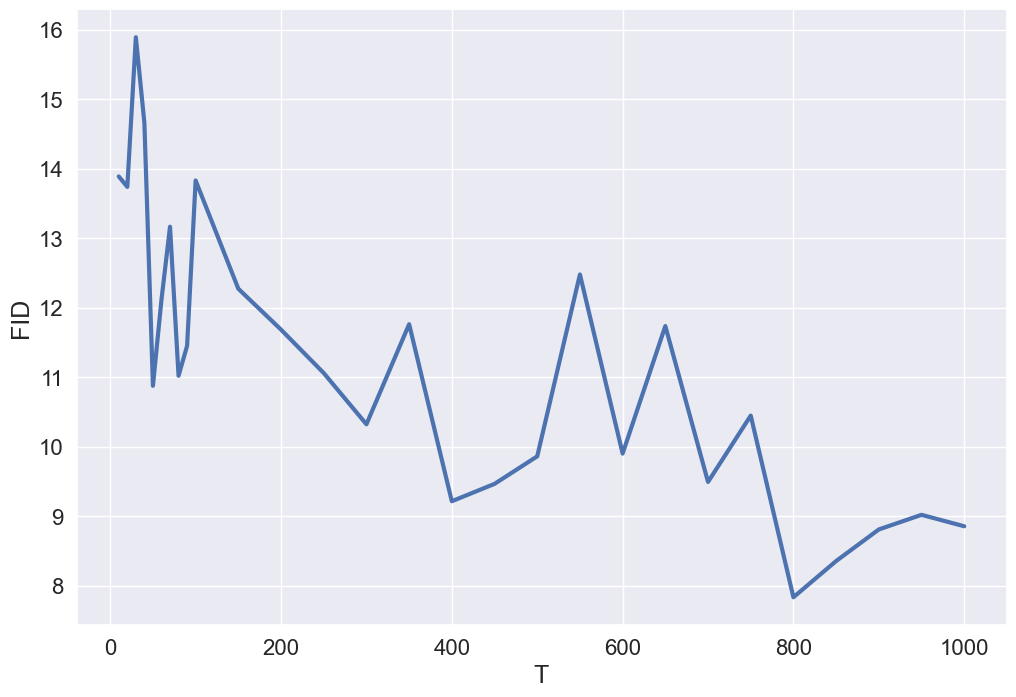
\includegraphics[scale = 0.4]{../code/DDPM_FID_FMNIST.png}}
	\caption{Зависимость FID от количества шагов для DDPM}\label{ddpm_fid}
\end{figure}

Как и ожидалось, качество семплов ) значительно повышается с ростом T, что видно на примерах, см. рис. \ref{ddpm_samples}.

\begin{figure}[H]
	\begin{subfigure}[h]{0.3\linewidth}
		\centering
		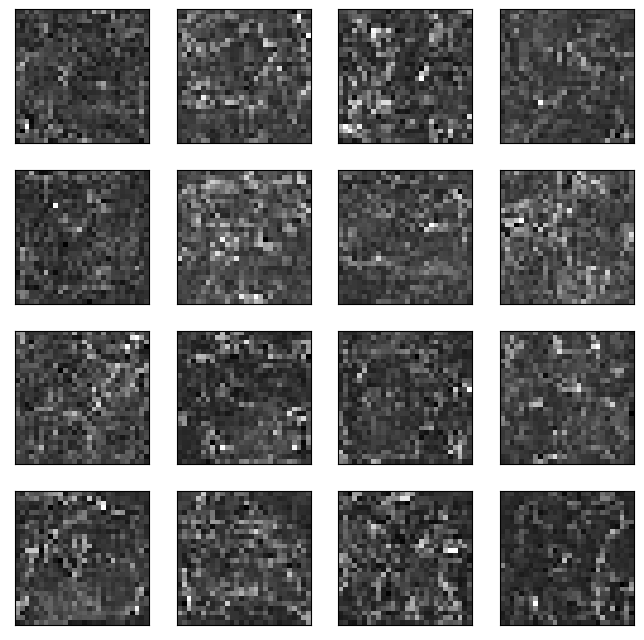
\includegraphics[scale=0.3]{../code/generated_DDPM_50.png}
		\caption{T = 50}
	\end{subfigure}
	\hfill
	\begin{subfigure}[h]{0.3\linewidth}
		\centering
		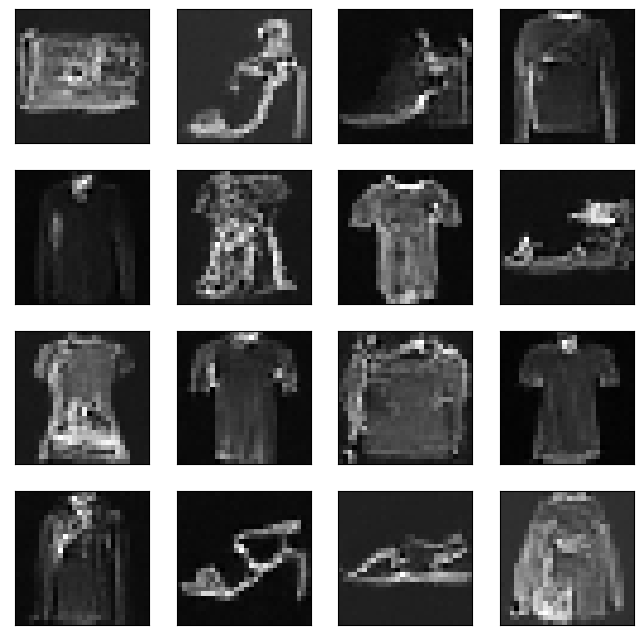
\includegraphics[scale=0.3]{../code/generated_DDPM_300.png}
		\caption{T = 300}
	\end{subfigure}
	\hfill
	\begin{subfigure}[h]{0.3\linewidth}
		\centering
		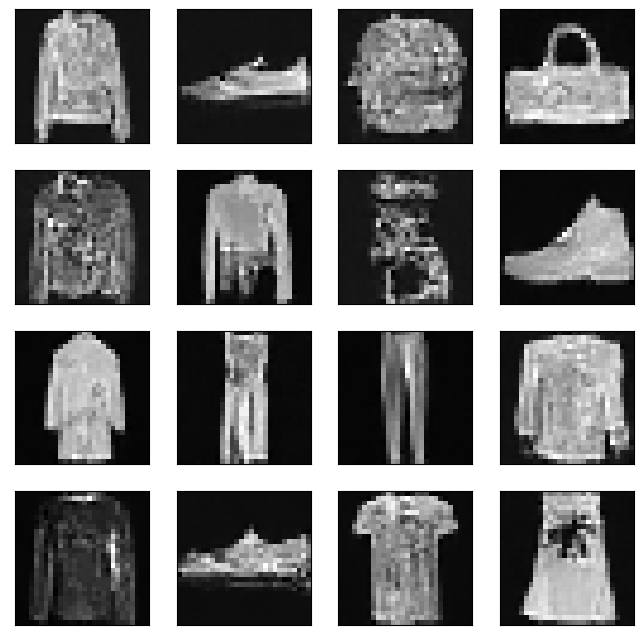
\includegraphics[scale=0.3]{../code/generated_DDPM_1000.png}
		\caption{T = 1000}
	\end{subfigure}
\caption{Семплы из DDPM для различных значений T}\label{ddpm_samples}
\end{figure}

\subsection{DDGAN}
Теперь заменим модель, используемую для диффузионного процесса на неявную модель. Для начала используем non-saturating GAN \cite{https://doi.org/10.48550/arxiv.1406.2661} как в оригинальной статье. Используем в качестве дискриминатора половину U-Net модели из базового эксперимента с дополнительным линейным выходным слоем, в качестве генератора аналогичный U-Net с дополнительными слоями эмбеддинга для латентной переменной. 

Целью использования неявной модели является существенное уменьшение числа шагов обратного процесса, поэтому будем рассматривать различные T от 1 до 10. Для них посчитаем FID, построим график (рис. \ref{ddgan_fid}) и рассмотрим сгенерированные моделью примеры. (рис. \ref{ddgan_samples})

\begin{figure}[H]	
	\centering{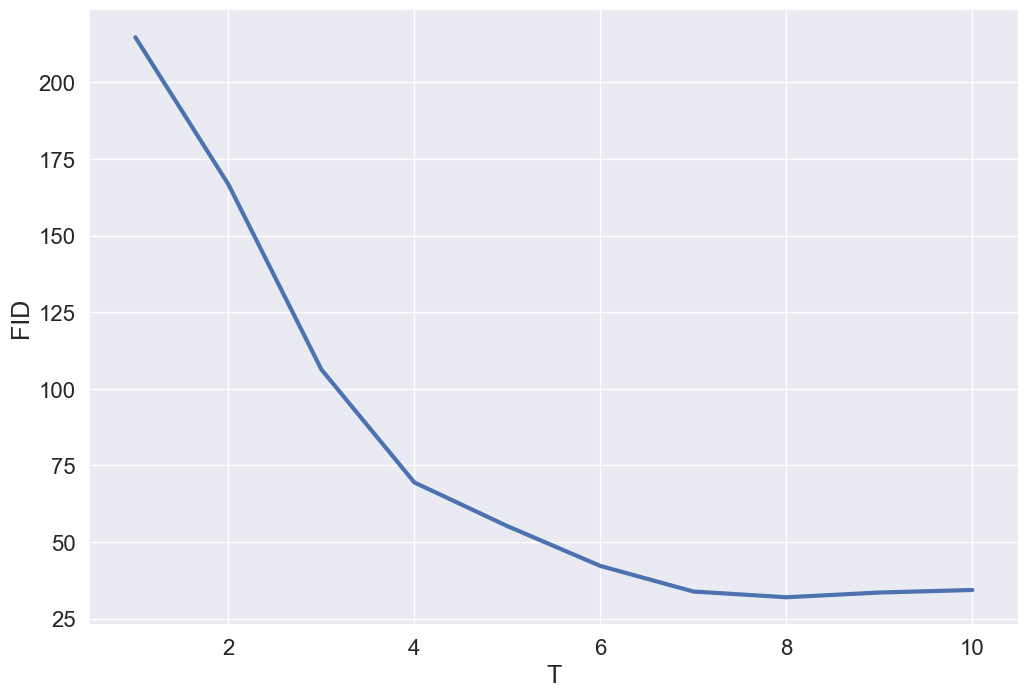
\includegraphics[scale = 0.4]{../code/DDGAN_FID_FMNIST.png}}
	\caption{Зависимость FID от количества шагов для DDGAN}\label{ddgan_fid}
\end{figure}

\begin{figure}[H]
	\begin{subfigure}[h]{0.3\linewidth}
		\centering
		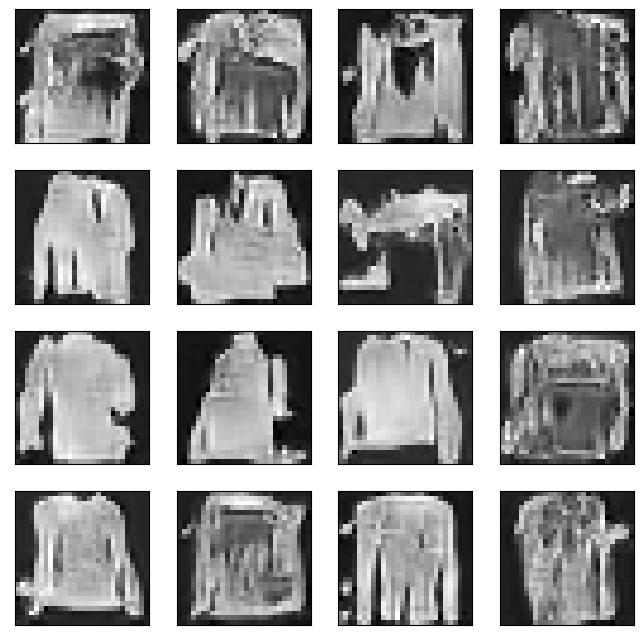
\includegraphics[scale=0.3]{../code/generated_DDGAN_3.png}
		\caption{T = 3}
	\end{subfigure}
	\hfill
	\begin{subfigure}[h]{0.3\linewidth}
		\centering
		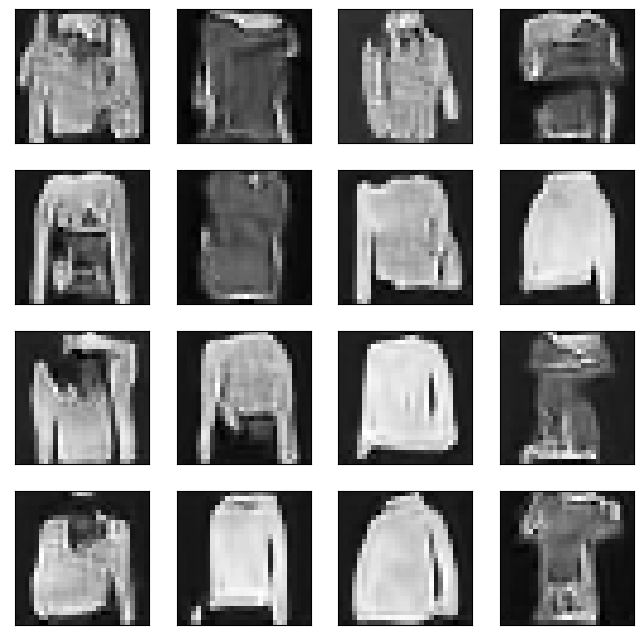
\includegraphics[scale=0.3]{../code/generated_DDGAN_5.png}
		\caption{T = 5}
	\end{subfigure}
	\hfill
	\begin{subfigure}[h]{0.3\linewidth}
		\centering
		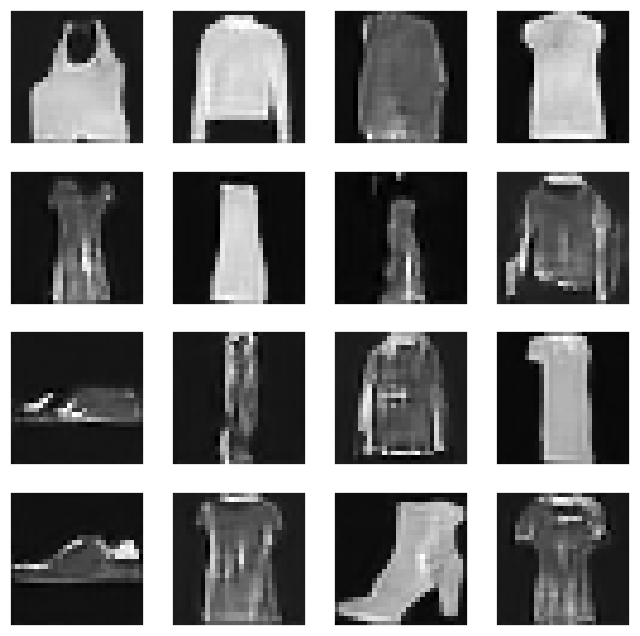
\includegraphics[scale=0.3]{../code/generated_DDGAN_10.png}
		\caption{T = 10}
	\end{subfigure}
	\caption{Семплы из DDGAN для различных значений T}\label{ddgan_samples}	
\end{figure}

\subsection{Альтернативные GAN модели}

Далее изменим постановку задачи минимизации, для соответствия другим схемам тренировки GAN моделей. 

Используем как и раньше 2 сверточных сети, тренируемых параллельно, изменяем лишь функции потерь для соответствия схеме минимизации определенной дивергенции, все также рассматриваем число шагов T от 1 до 10. Для трех получившихся моделей построим графики зависимости FID-score от T (рис. \ref{ddgan_all_fid}) и приведем примеры семплов (рис. \ref{ddgan_h2_samples}, \ref{ddgan_rkl_samples}, \ref{ddgan_tv_samples}).

\begin{figure}[H]	
	\centering{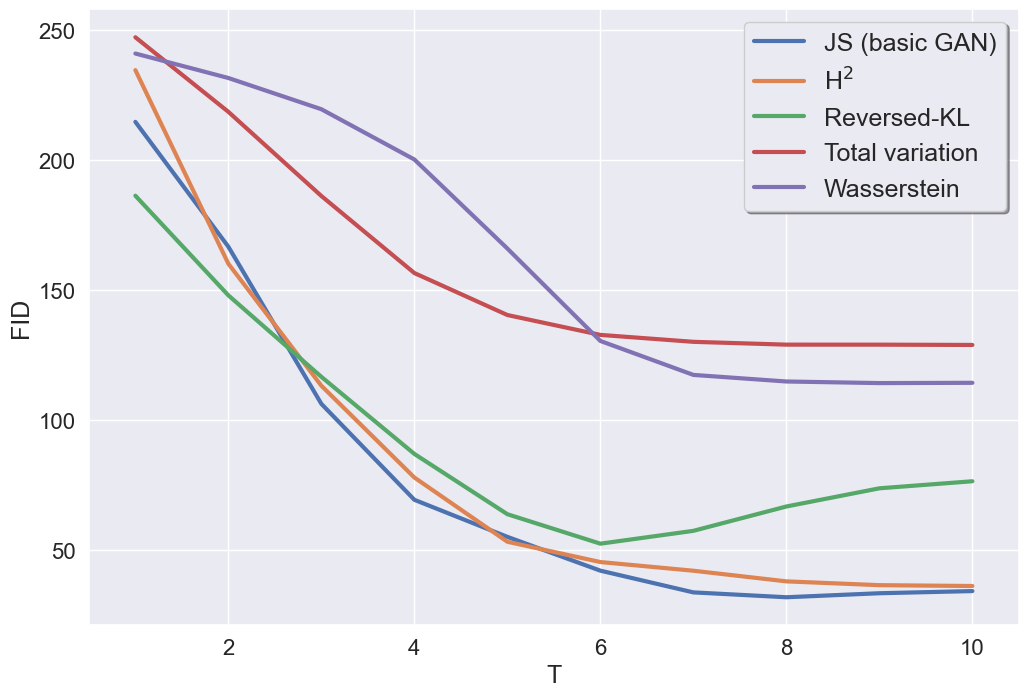
\includegraphics[scale = 0.4]{../code/DDGAN_ALL_FID_FMNIST.png}}
	\caption{Зависимость FID от количества шагов для различных GAN моделей в диффузионной сети}\label{ddgan_all_fid}
\end{figure}

\begin{figure}[H]
	\begin{subfigure}[h]{0.3\linewidth}
		\centering
		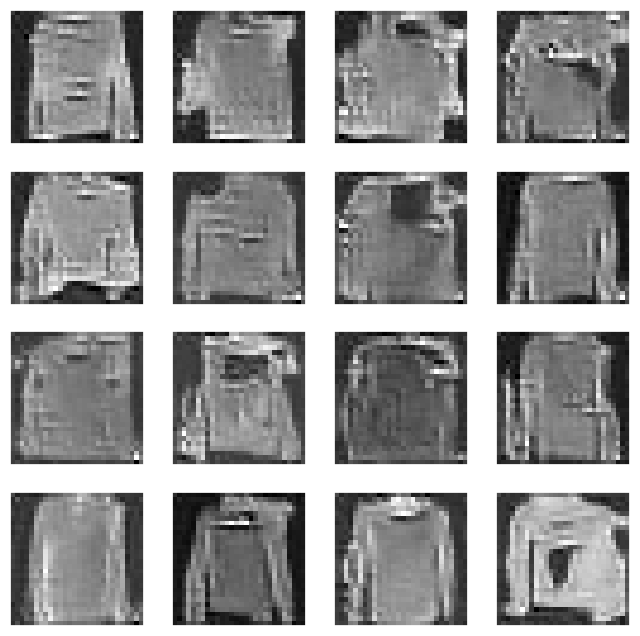
\includegraphics[scale=0.3]{../code/generated_DDGAN_h2_3.png}
		\caption{T = 3}
	\end{subfigure}
	\hfill
	\begin{subfigure}[h]{0.3\linewidth}
		\centering
		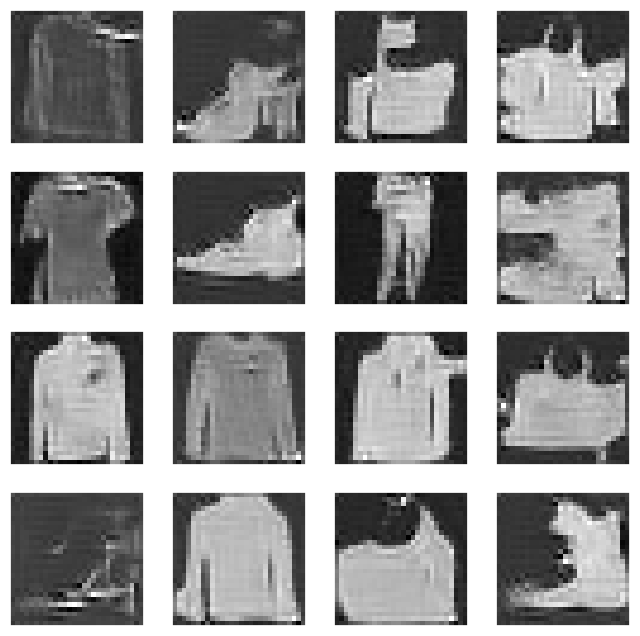
\includegraphics[scale=0.3]{../code/generated_DDGAN_h2_5.png}
		\caption{T = 5}
	\end{subfigure}
	\hfill
	\begin{subfigure}[h]{0.3\linewidth}
		\centering
		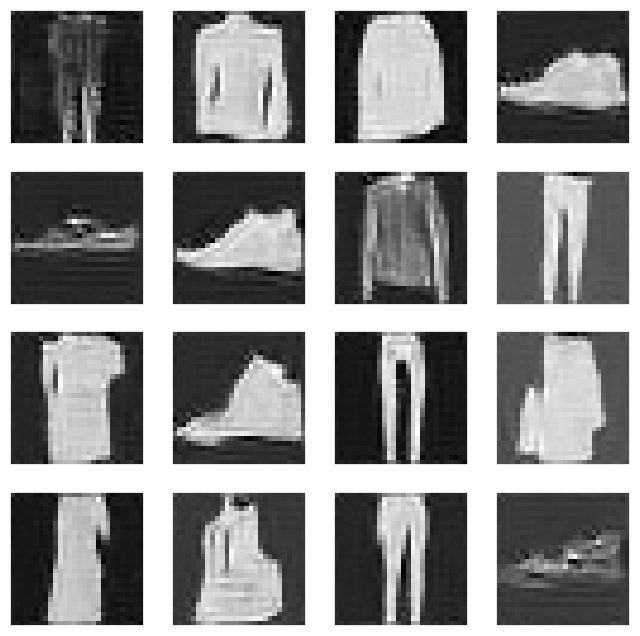
\includegraphics[scale=0.3]{../code/generated_DDGAN_h2_10.png}
		\caption{T = 10}
	\end{subfigure}
	\caption{Семплы из DDGAN c $H^2$}\label{ddgan_h2_samples}	
\end{figure}

\begin{figure}[H]
	\begin{subfigure}[h]{0.3\linewidth}
		\centering
		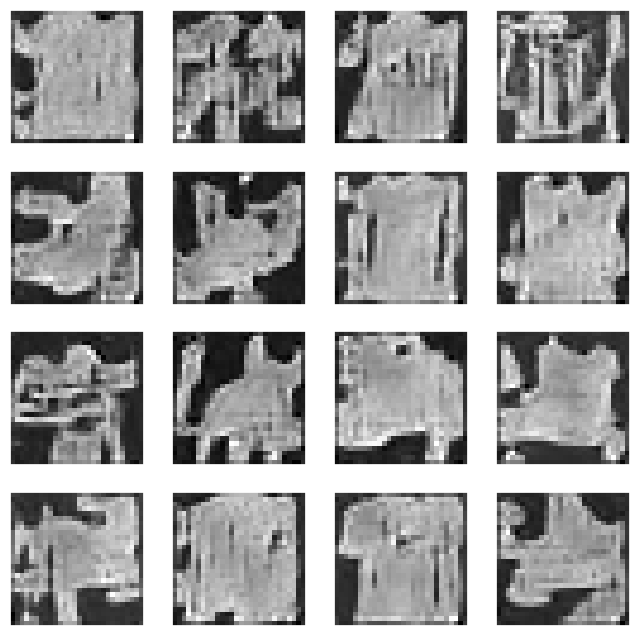
\includegraphics[scale=0.3]{../code/generated_DDGAN_rkl_3.png}
		\caption{T = 3}
	\end{subfigure}
	\hfill
	\begin{subfigure}[h]{0.3\linewidth}
		\centering
		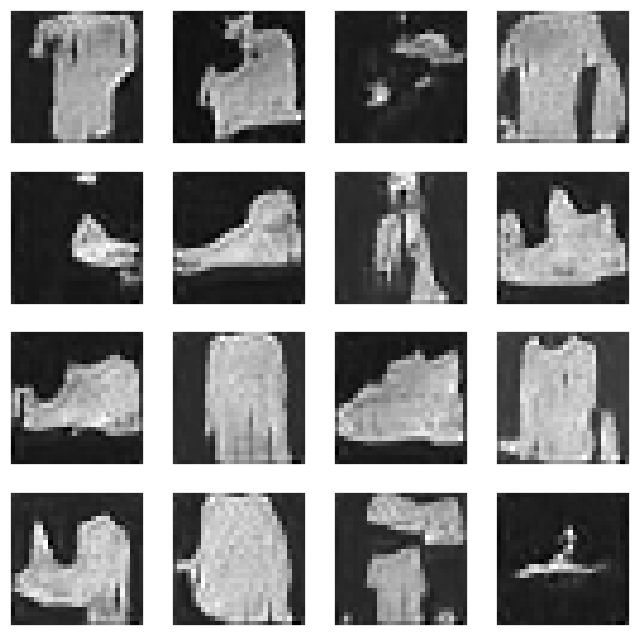
\includegraphics[scale=0.3]{../code/generated_DDGAN_rkl_5.png}
		\caption{T = 5}
	\end{subfigure}
	\hfill
	\begin{subfigure}[h]{0.3\linewidth}
		\centering
		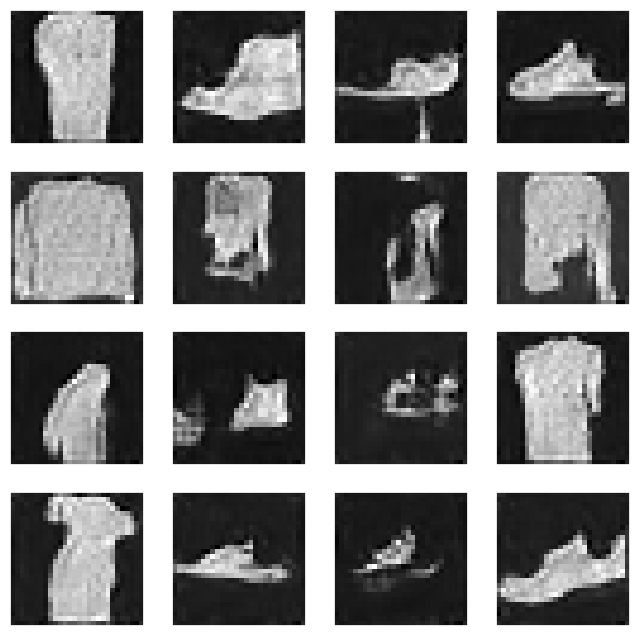
\includegraphics[scale=0.3]{../code/generated_DDGAN_rkl_10.png}
		\caption{T = 10}
	\end{subfigure}
	\caption{Семплы из DDGAN c reversed-KL}\label{ddgan_rkl_samples}	
\end{figure}

\begin{figure}[H]
	\begin{subfigure}[h]{0.3\linewidth}
		\centering
		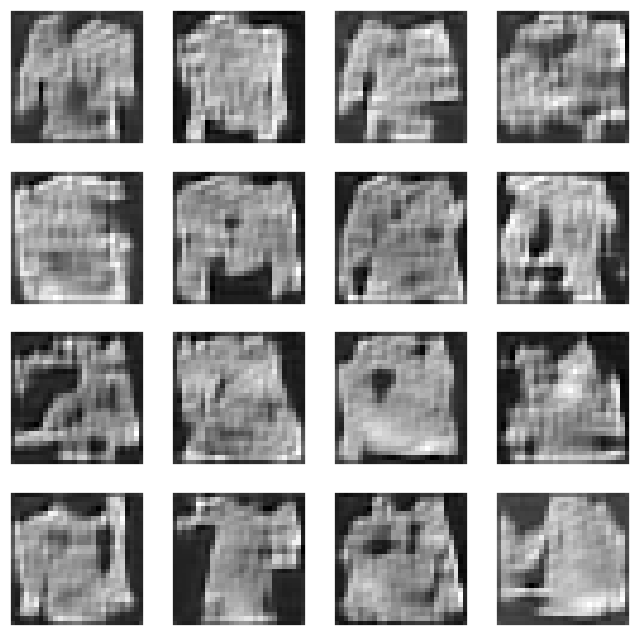
\includegraphics[scale=0.3]{../code/generated_DDGAN_tv_3.png}
		\caption{T = 3}
	\end{subfigure}
	\hfill
	\begin{subfigure}[h]{0.3\linewidth}
		\centering
		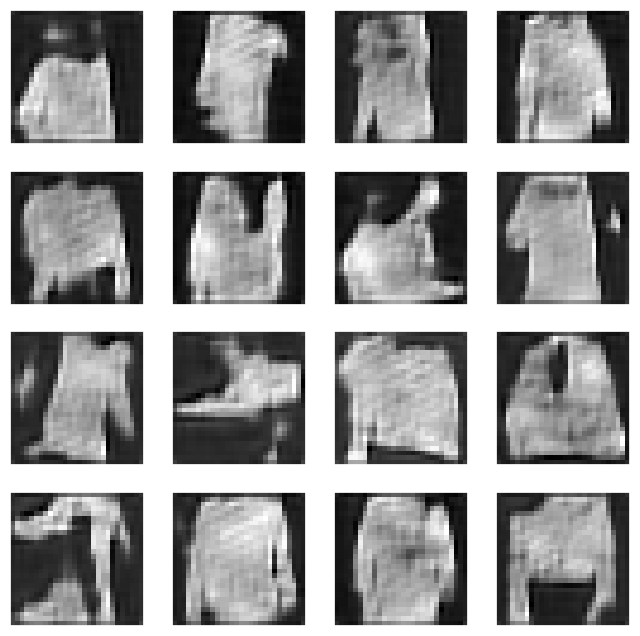
\includegraphics[scale=0.3]{../code/generated_DDGAN_tv_5.png}
		\caption{T = 5}
	\end{subfigure}
	\hfill
	\begin{subfigure}[h]{0.3\linewidth}
		\centering
		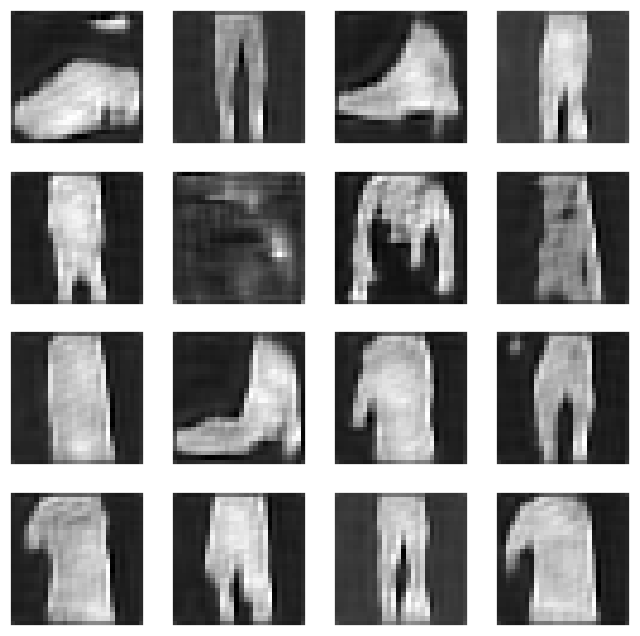
\includegraphics[scale=0.3]{../code/generated_DDGAN_tv_10.png}
		\caption{T = 10}
	\end{subfigure}
	\caption{Семплы из DDGAN c total variation}\label{ddgan_tv_samples}	
\end{figure}



\bibliographystyle{plain}
\bibliography{references}

\end{document}